%% VRL survey, expanded version for ACM Computing Surveys.
%% Submission format: acmart manuscript (single column, review-friendly).
%% Switch to [acmsmall,screen] for the final version per ACM instructions.
\documentclass[manuscript,screen,review]{acmart}

\usepackage{tikz}
\usepackage[edges]{forest}
\usepackage{booktabs}
\usepackage{multirow}
\usepackage{colortbl}
\usepackage{adjustbox}
\usepackage{enumitem}
\usepackage{xcolor}
\usepackage{pifont}
\usepackage{array}
\usepackage{tabularx}
\usepackage{longtable}
\usepackage{xspace}
\usetikzlibrary{trees,shapes,calc,arrows.meta,positioning}

\newcommand{\verbalrl}{Verbal RL\xspace}
\newcommand{\vrl}{VRL\xspace}

%% Draft-phase margin notes; zero usages remain as of the Phase F pass.
%% Kept deliberately for the revision cycle; strip before submission.
\newcommand{\todonote}[1]{\textcolor{red}{[TODO: #1]}}

\citestyle{acmauthoryear}
\setcopyright{none}

\begin{document}

\title{The Rise of Verbal Reinforcement Learning: A Survey}

%% Authors withheld in working draft; fill at submission:
%% Kshitij Tayal, Arun Sharma, Genta Indra Winata, Anirban Das, Sambit Sahu
\author{Anonymous}
\affiliation{\institution{Working draft}\city{Minneapolis}\country{USA}}

\begin{abstract}
Large language models turned natural language from a task description into a learning signal: critiques, rubrics, reflections, and debates now steer agents where scalar rewards once did. We survey this practice as verbal reinforcement learning (VRL), organizing methods by the signal itself: what linguistic artifact is consumed, which decision-problem component it modifies, and when it takes effect. A formal framework with explicit inclusion criteria separates VRL from scalarized preference learning. We synthesize credit assignment for verbal signals, the verbal reward stack, language-space optimizers, embodied settings, evaluation, and feedback-channel safety, and distill decision rules for practitioners.
\end{abstract}

\maketitle

\section{Introduction}
\label{sec:intro}

\begin{figure}[!th]
    \centering
    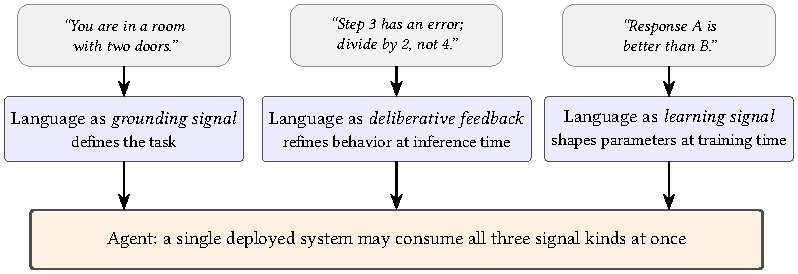
\includegraphics[width=\linewidth]{paper_images/generated/overview.pdf}
    \Description{Three example language signals map to grounding, deliberative feedback, and learning. Arrows from all three roles point to one agent, showing that a single system may consume the roles together.}
    \caption{Language plays three complementary roles as a signal in agentic systems: grounding the task and environment, scaffolding intermediate deliberation, and serving as a learning signal for training. The three roles classify signals, not system stages; a single deployed system may consume all three (\S\ref{sec:taxonomy}).}
    \label{fig:overview}
\end{figure}

Classical reinforcement learning assumes a specified environment, action space, and reward. Its landmark successes therefore depend on substantial domain engineering and on objectives whose optima match their designers' intent \citep{mnih2015human,silver2016mastering,vamplew2021scalarrewardenoughresponse}. This specification burden is most acute for ambiguous, context-dependent tasks that resist scalar rewards \citep{amodei2016concrete}.

Large language models open a second supervisory channel: language can express task intent, diagnose an output, preserve a lesson, or supply training feedback in a form an agent can consume directly \citep{brown2020language,achiam2023gpt,madaan2023selfrefine}. The central question is no longer only how to derive a better scalar reward, but when retaining the structure of a critique, rubric, or instruction changes what can be learned.

We call the resulting family \textbf{verbal reinforcement learning (VRL)} and impose two membership criteria. First, feedback is expressed in natural language and its linguistic structure is functionally consumed, rather than collapsed to a scalar or preference bit before use. Second, it participates in an improvement loop through output revision, memory write, parameter update, or construction of a decision-problem component that later drives such an update. Both criteria are required. Plain instruction following fails the second. Vanilla RLHF \citep{christiano2017deep,ouyang2022training} and DPO \citep{rafailov2023direct} fail the first because the rationale is discarded before learning. Language-conditioned RL treats language as policy input while an ordinary scalar reward drives improvement. Reward-code generation remains inside the fence because a compiler consumes the language before the resulting reward drives optimization. Only feedback must be textual, so agents with visual observations remain in scope when their corrections are verbal (\S\ref{sec:embodied}). Section~\ref{sec:framework} formalizes this fence.

We organize qualifying signals by when they take effect and what they modify. A \emph{grounding signal} defines goals, states, actions, or reward structure at problem-definition time. \emph{Deliberative feedback} revises context, output, or memory during inference without changing weights. A \emph{learning signal} changes parameters or training data. These are roles of signals, not mutually exclusive system types or lifecycle stages: one agent can consume all three. Existing surveys usually organize by correction mechanism, agent component, or optimization family \citep{pan2023automatically,zhang2025survey,wang2024reinforcement}; our signal-centric axis instead connects problem definition, inference, training, credit assignment, evaluation, and feedback-channel safety.

This article makes four contributions.
\begin{enumerate}
    \item \textbf{Formalism and taxonomy.} A language-augmented decision framework locates linguistic artifacts at six entry points, while an explicit assignment rule resolves hybrid methods by the component modified when a signal takes effect (\S\ref{sec:framework}, \S\ref{sec:taxonomy}).
    \item \textbf{Mechanism synthesis.} We connect the three pillars to the verbal reward stack, credit assignment, and language-space optimization, distinguishing outcome, process, token, context, memory, and parameter updates (\S\ref{sec:rewardstack}, \S\ref{sec:credit}, \S\ref{sec:optimizers}).
    \item \textbf{Evaluation and safety.} We separate feedback quality from feedback utilization and analyze attacks and defenses at the feedback channel rather than treating the signal as trusted input (\S\ref{sec:evaluation}, \S\ref{sec:safety}).
    \item \textbf{Practice and positioning.} We provide mechanism-selection rules, compare eighteen neighboring surveys and frameworks on fixed dimensions, and derive a focused research agenda (\S\ref{sec:practitioner}).
\end{enumerate}

Sections~\ref{sec:framework} and~\ref{sec:taxonomy} establish the formalism and taxonomy; Sections~\ref{sec:grounding} through~\ref{sec:learning} develop the pillars. The remaining sections treat rewards, credit, optimization, embodiment, evaluation, safety, and practitioner decisions before Section~\ref{sec:conclusion} concludes.

\section{A Formal Framework for Verbal Reinforcement Learning}
\label{sec:framework}

The methods surveyed in later sections share a decision-theoretic skeleton but attach language to it in different places. This section fixes that skeleton once. We define a language-augmented partially observable Markov decision process (POMDP), enumerate the points at which a linguistic artifact, written $\ell$ throughout, can enter it, and introduce an improvement operator $\mathcal{I}$ whose three realizations underpin the taxonomy of \S\ref{sec:taxonomy}. We then restate the two criteria that fence verbal reinforcement learning (VRL) off from adjacent paradigms, trace the genealogy of the term, and close by stating plainly which formal guarantees exist and which do not.

\subsection{The Language-Augmented Decision Process}
\label{subsec:setting}

We begin from a standard POMDP $\mathcal{M} = (\mathcal{S}, \mathcal{A}, \Omega, T, R, O, \gamma)$ \citep{kaelbling1998planning}: a Markov decision process with state space $\mathcal{S}$, action space $\mathcal{A}$, transition kernel $T$, reward function $R$, and discount $\gamma$ \citep{sutton2018reinforcement}, made partially observable by an observation space $\Omega$ and an observation function $O$ through which the agent perceives state only indirectly. Let $\mathcal{L}$ denote the set of finite natural-language strings. A \emph{linguistic artifact} $\ell \in \mathcal{L}$ is any string that the system produces or consumes as a signal: a task description, a critique, a rationale, a stored lesson, or a generated fragment of reward code. The agent is a configuration $\kappa = (\theta, c, m)$ comprising model parameters $\theta$, a working context $c$ (the prompt and any in-context material), and a persistent memory $m$; the policy $\pi_{\kappa}$ maps interaction histories to distributions over actions, which in language settings are themselves strings.

The construct that distinguishes VRL from ordinary language-conditioned control is the \emph{improvement operator}
\begin{equation}
\mathcal{I} : (\kappa, \ell) \longmapsto \kappa',
\label{eq:improvement}
\end{equation}
which consumes an artifact and returns a modified agent configuration. Three minimal realizations recur throughout the literature. An \emph{output revision} alters only $c$: a critique is appended to the context and the agent regenerates, as in iterative self-refinement \citep{madaan2023selfrefine}, and the effect vanishes when the episode ends. A \emph{memory write} alters only $m$: a reflection or distilled lesson is stored and retrieved in later episodes \citep{shinn2023reflexion,zhou2025memento}, so the effect persists without touching the weights. A \emph{parameter update} alters only $\theta$: the artifact, or a signal derived from it, changes the model itself and therefore all future behavior. Composite operators exist; Constitutional AI first revises outputs against written principles and then trains on the revisions, chaining the first and third realizations \citep{bai2022constitutional}.

Language can enter this augmented process at six points.
\begin{enumerate}[label=(\roman*),leftmargin=2.2em,itemsep=0.2em]
    \item \emph{Goal specification.} A task description $g \in \mathcal{L}$ defines what counts as success, often without any executable reward; the true objective is latent and reaches the agent only through language, the setting formalized as learning from language feedback in \S\ref{subsec:guarantees}.
    \item \emph{State and observation.} Observations may be linguistic (text environments, tool outputs, error traces) or verbalized descriptions of non-linguistic state; language then acts as a state abstraction whose fidelity bounds what the policy can distinguish (\S\ref{sec:grounding}).
    \item \emph{Action prior.} Instructions and subgoals reshape the distribution over actions before any learning occurs; in hierarchical designs an LLM planner emits subgoals in $\mathcal{L}$ that a low-level actor must realize \citep{he2024words}.
    \item \emph{Reward.} Timing is essential here. At \emph{specification time}, a generator compiles $\ell$ into an executable reward function $\hat{R} = C(\ell)$, as in reward-code generation \citep{ma2024eureka}: the linguistic structure is consumed by the compiler even though the resulting function emits scalars. At \emph{runtime}, a judge model maps trajectories to evaluations, verbal or scalar, on the fly \citep{zheng2023judging}. \S\ref{sec:rewardstack} develops this stack in full.
    \item \emph{Transition prior.} Pretrained linguistic knowledge supplies an implicit world model: predictions about the consequences of an action can be elicited in language before, or instead of, environment interaction \citep{he2024words}.
    \item \emph{The improvement operator.} Critiques, reflections, and preference rationales serve as the argument $\ell$ in Eq.~\eqref{eq:improvement}; this entry point hosts the second and third pillars of the taxonomy.
\end{enumerate}

The taxonomy of \S\ref{sec:taxonomy} classifies a signal by which of these points it acts on and, for the last, by which realization of $\mathcal{I}$ consumes it. Signals that instantiate the goal, observation, action-prior, or reward components of $\mathcal{M}$, points (i) through (iv), act at problem-definition time and constitute the grounding signal of \S\ref{sec:grounding}; artifacts consumed by output revision or memory write at inference time constitute deliberative feedback (\S\ref{sec:deliberative}); artifacts distilled into parameter updates constitute the learning signal (\S\ref{sec:learning}). Point (v) is the exception, and we state it plainly: a transition prior is not written down when the problem is defined but elicited from the pretrained model during interaction, and no method we survey consumes a linguistic artifact at this point. The taxonomy therefore operationalizes five of the six entry points; the transition prior enters the survey only through the theoretical analysis of \S\ref{subsec:guarantees} and stands as an entry point the literature has yet to occupy. Two caveats keep the formalism honest. First, the framework is an organizing lens, not a claim that every method admits a POMDP formulation, and the boundary is concrete. Open-ended web and tool-use tasks specify no transition kernel and no reward function; success is adjudicated post hoc by a judge or a human, so $T$ and $R$ are notational conveniences rather than defined objects. Dialogue sets the agent against an interlocutor whose state admits no compact Markovian summary. And once memory writes alter $m$, later episodes unfold in an environment the agent itself has changed, breaking stationarity (\S\ref{sec:credit}). In these regimes we use the formalism as vocabulary and do not import its theorems. Second, multi-turn language interaction typically carries a two-level structure, an utterance-level decision process layered over a token-level one, and both benchmark design and algorithm design increasingly make this decomposition explicit \citep{abdulhai2023lmrl,zhou2024archer}.

\subsection{The Definitional Fence}
\label{subsec:fence}

With this notation, the definition of \S\ref{sec:intro} can be restated precisely. A method belongs to VRL if and only if (i) the feedback is expressed in natural language, whether self-generated, provided by a human, or produced by an external tool or model, and its linguistic structure is functionally consumed by the agent rather than being collapsed to a scalar or preference bit before use; and (ii) the feedback participates in an improvement loop, that is, an output revision, a memory write, or a parameter update.

Criterion (i) can be phrased through a scalarization map $\sigma : \mathcal{L} \to \mathbb{R}^{k}$: if replacing $\ell$ by $\sigma(\ell)$ everywhere leaves the method's behavior unchanged, the linguistic structure was not functionally consumed and the criterion fails. Two terms in this test need pinning down. \emph{Unchanged} means distributional, not token-level, invariance: the distribution over updated configurations $\kappa'$, and hence over subsequent behavior on the method's own task distribution, is the same under $\ell$ and $\sigma(\ell)$. \emph{Small $k$} means that $k$ is fixed by the method rather than growing with the content of $\ell$, and it is counted per judged unit: a preference bit, a grade, a fixed vector of rubric scores, or one score per reasoning step is a scalarization, however many steps the judged trajectory contains; retaining the text is not. Criterion (ii) requires that $\ell$ appear as the argument of $\mathcal{I}$, or construct a component of $\mathcal{M}$ that subsequently drives $\mathcal{I}$, as a compiled reward function does.

The test is still a counterfactual, and \S\ref{subsec:guarantees} concedes that no measured quantity certifies it, so we state the inspection procedure used to adjudicate membership throughout this survey. For each method we trace the artifact from its producer to the operator that consumes it and mark the \emph{scalarization boundary}, the point at which language collapses into the numbers the learner receives; \S\ref{sec:rewardstack} develops this construct in full. What crosses the interface to $\mathcal{I}$ decides the case. Criterion (i) holds when some consumer downstream of the artifact reads its structure: a compiler that parses $\ell$ into reward code \citep{ma2024eureka}, a reviser that conditions on a critique \citep{madaan2023selfrefine}, a retriever that matches stored lessons \citep{shinn2023reflexion}, or a training loss computed over the text itself. It fails when the only consumer is a judge or annotator whose output is the scalar. The intermediate formats that dominate practice resolve by the same trace. A rationale-annotated preference qualifies when the rationale enters the training distribution or a revision loop, and does not when only the bit survives. A step-level critique qualifies when downstream machinery converts its content into credit, as when critique text is converted into token-level credits \citep{xie2025capo}, and reduces to process supervision when only per-step scores survive \citep{lightman2024let}. A generative process reward model reasons in language before scoring \citep{zhao2025genprm}; its boundary sits at verdict emission, so the linguistic structure is consumed inside the reward computation while the optimizer receives per-step scalars, the same route by which compiled rewards enter, unless the critique is separately routed into revision or critique-level supervision \citep{wang2026reward}, which moves the boundary later. The trace reduces the counterfactual to a question about dataflow; the residual judgment is empirical, namely whether a consumer positioned to read the structure in fact exploits it, and only the missing certificate of \S\ref{subsec:guarantees} would replace that judgment with a measurement. \S\ref{sec:learning} arranges learning-signal methods along the resulting compression spectrum, from methods that keep $\ell$ verbatim in the training distribution to methods that retain only $\sigma(\ell)$.

Both criteria are required, and each excludes a neighboring paradigm. Plain instruction following fails criterion (ii): the instruction conditions the policy, but nothing is revised, written, or updated, so no improvement loop exists. Vanilla RLHF \citep{ouyang2022training} and DPO \citep{rafailov2023direct} fail criterion (i): the annotator's verbal judgment is collapsed to a preference bit before it reaches the update, and the content that would make the signal verbal, the reason one response beats another, is discarded; we treat these methods only as the scalar endpoint of the compression spectrum. Language-conditioned RL \citep{luketina2019survey} treats language as an input to the policy rather than as feedback on its behavior; improvement is driven by an ordinary scalar reward, so language never enters the loop of criterion (ii). One boundary case the criteria settle explicitly: language consumed at specification time to construct a reward function satisfies criterion (i), because the generator exploits the full structure of $\ell$, and criterion (ii) through the training loop the constructed reward drives \citep{ma2024eureka}. Finally, the criteria fix the modality scope: the feedback signal is natural-language text, while observations may be non-textual, as in embodied settings where verbal corrections accompany visual state (\S\ref{sec:embodied}).

\subsection{Genealogy and Neighboring Formalisms}
\label{subsec:genealogy}

The phrase predates machine learning: in mid-twentieth-century behavioral psychology, verbal reinforcement denoted approving utterances an experimenter used to shape a subject's responses \citep{greenspoon1955reinforcing,krasner1958studies}. In the LLM era the term was introduced by \citet{shinn2023reflexion}, whose subtitle, ``Language Agents with Verbal Reinforcement Learning,'' named a specific mechanism: agents reflect verbally on task feedback and keep those reflections in an episodic buffer that guides later attempts, an instance of $\mathcal{I}$ realized as a memory write. We generalize the term deliberately to any method satisfying the two criteria above, flagging the departure from the original, narrower sense.

The closest formal ancestor of our framework is Natural Language Reinforcement Learning \citep{feng2024natural}, which extends the core objects of RL into language counterparts: the language value function replaces a scalar estimate with a narrative articulating the rationale behind an evaluation, and Bellman backups and policy iteration are redefined analogously, with LLMs implementing the resulting operators. Its authors argue that scalar value restricts an agent's understanding of its environment and report gains in effectiveness and interpretability on multi-step agentic tasks. In our notation, NLRL relocates the codomain of the value function from $\mathbb{R}$ to $\mathcal{L}$; the contribution is a framework, not an overview of the field, and the language-space optimizers of \S\ref{sec:optimizers} build directly on this move.

A second neighbor replaces reward maximization with conditional generation: the feedback-conditional policy \citep{luo2025fcp} learns the posterior over responses given feedback and bootstraps online under positive feedback conditions. Its motivating argument, that scalarizing nuanced feedback discards richness, is the probabilistic form of criterion (i): the feedback string survives into the training objective itself.

A third neighbor makes memory the learned object: Memento \citep{zhou2025memento} casts continual adaptation as a memory-augmented Markov decision process (M-MDP) in which the policy improves by rewriting and retrieving episodic cases, with the underlying LLM never fine-tuned. The M-MDP makes precise the sense in which memory is persistent state rather than inference-time scaffolding, the boundary question experiential memory poses for the taxonomy (\S\ref{sec:taxonomy}); the credit-assignment problem that memory writes create \citep{yan2026memoryr2} returns in \S\ref{sec:credit}.

Two earlier organizing efforts situate ours. Language grounding in RL predates LLMs \citep{branavan2009reinforcement}, and \citet{luketina2019survey} surveyed that first wave, dividing it into language-conditional RL, where language is part of the problem, and language-assisted RL, where language aids learning. Our framework is the LLM-era successor to that division: language is no longer only an input or an auxiliary knowledge source but the medium of evaluation and revision, and the policy itself is a language model, so every entry point of \S\ref{subsec:setting} is realizable by a single substrate. CoALA \citep{sumers2023cognitive} instead organizes agent computation into memory modules, action spaces, and decision cycles. The two lenses are complementary: CoALA says where computation and storage live inside an agent, whereas we classify the signals that flow through it, and a single CoALA-style architecture can host grounding, deliberative, and learning signals simultaneously (\S\ref{sec:taxonomy}).

\subsection{What Is Formally Guaranteed, and What Is Not}
\label{subsec:guarantees}

Formal results exist, but they are recent and localized. \citet{xu2025formalizing} give the first principled formalization of the learning-from-language-feedback (LLF) problem: sufficient assumptions under which learning is possible even though rewards are latent, a complexity measure, the transfer eluder dimension, that quantifies how informative feedback is, and a no-regret algorithm, HELiX, whose guarantees scale with that dimension. Their separation result is the theoretical warrant for the field's premise: learning from rich language feedback can be exponentially faster than learning from reward alone. Complementing this, \citet{he2024words} analyze a hierarchical planner and actor system inside a POMDP and prove that, under assumptions on the pretraining distribution, an LLM planner performs Bayesian aggregated imitation learning through in-context learning; naive execution of the imitated subgoals incurs linear regret, and epsilon-greedy exploration on top of the imitator restores sublinear regret when the pretraining error is small. The lesson generalizes: language-mediated hierarchies do not escape the exploration problem. At the level of problem statements rather than theorems, LLF-Bench operationalizes the setting, replacing numeric reward with natural-language instructions and feedback and randomizing verbalizations so that agents must genuinely learn from the feedback channel \citep{cheng2023llfbench}.

The list of what is missing is longer. There is no convergence or contraction analysis for language-space Bellman operators, and to our knowledge no analogue of the policy improvement theorem exists for $\mathcal{I}$ in any of its realizations: nothing certifies that a revision, a memory write, or a critique-driven update makes the policy better rather than differently biased. Existing regret results assume that feedback carries reliable information about a latent ground-truth objective; no bound covers self-generated feedback that shares the biases of the policy it evaluates, the regime in which most deliberative methods operate (\S\ref{sec:safety}). The separation of \citet{xu2025formalizing} contrasts the ends of the compression spectrum, rich feedback against scalar reward; no complexity characterization exists for the intermediate formats that dominate practice, step-level critiques or rationale-annotated preferences. Criterion (i) itself lacks a certificate: no measurable quantity attests how much of an artifact's linguistic structure a learner actually exploits, so the fence must be applied by the boundary trace of \S\ref{subsec:fence}, which settles what a mechanism could read but not what it in fact uses. And no guarantee yet addresses noisy, adversarial, or strategically generated feedback channels. These gaps recur as concrete agenda items in \S\ref{sec:practitioner}.

The vocabulary of this section, $\ell$ for the linguistic artifact, $\kappa$ for the agent configuration, $\mathcal{I}$ for the improvement operator, and $\sigma$ for scalarization, does most of its work here, in the entry points, the fence, and the guarantees above; the later chapters inherit the distinctions rather than the symbols. The taxonomy of \S\ref{sec:taxonomy} rests on the mapping of \S\ref{subsec:setting}: entry points (i) through (iv) become its four grounding cells, the three realizations of $\mathcal{I}$ separate deliberative feedback from the learning signal, and the transition prior stands as the unoccupied sixth coordinate. The notation returns where an argument needs it, as $\sigma(\ell)$ does in the fence adjudication of \S\ref{sec:learning} and the credit-assignment analysis of \S\ref{sec:credit}; elsewhere the pillar chapters carry these distinctions in prose.

\section{Taxonomy}
\label{sec:taxonomy}
% BRIEF: upgrade of paper-acl/new_section/taxonomy.tex. Keep the three pillars as
% signal-classification (where a signal acts), NOT a lifecycle loop. Add: explicit
% assignment rule (placed by what the signal modifies at the moment it takes effect);
% hybrid-cases table (reward-code generation, experiential memory, Constitutional AI,
% critique-distillation) with multi-pillar tags; the coding-agent example reframed as
% one system consuming signals in three regimes. Fixes weaknesses (c) and Q27s-3.
\todonote{Draft; port pillar-overview table from ACL version.}

\section{Pillar 1: Language as Grounding Signal}
\label{sec:pillar1}
% BRIEF: deepen paper-acl/new_section/pillar_1.tex (goal/state/action grounding,
% reward-code generation). Add: the specification-time-consumption clarification;
% synthesis paragraph (shared failure modes: grounding gap, compositionality; when this
% pillar is the right tool). Reward-code cell cross-references S7.
\todonote{Port ACL text, deepen with T1/T6 notes.}

\section{Pillar 2: Language as Deliberative Feedback}
\label{sec:pillar2}
% BRIEF: deepen paper-acl/new_section/pillar_2.tex. Cells: self-critique, externally
% grounded critique (tools), multi-agent debate (T5), experiential memory (T4, positioned
% against dedicated memory surveys), evaluator-feedback-within-search (renamed per Q27s-6;
% inclusion criterion = linguistic evaluator signal, not the search procedure). Synthesis
% paragraph: feedback quality, circularity, compute; when this pillar wins.
\todonote{Port ACL text, deepen with T4/T5 notes.}

\section{Pillar 3: Language as Learning Signal}
\label{sec:learning}

The third pillar covers signals that persist through parameter updates. We organize its methods by how much linguistic structure survives into training. Feedback-conditioned modeling retains an entire critique; self-improvement uses feedback to filter generated data; trained critics and multi-agent learning optimize the producer of feedback; process supervision localizes judgments to steps; and preference shaping compresses a judgment to one comparative bit. Richer signals preserve actionable information but require a learner capable of consuming text, while scalar compression enables mature optimization machinery at the cost of expressiveness. An orthogonal online-offline axis records whether feedback is collected from the current policy or inherited from a fixed corpus. Figure~\ref{fig:compression-spectrum} summarizes both distinctions.

\begin{figure}[!t]
    \centering
    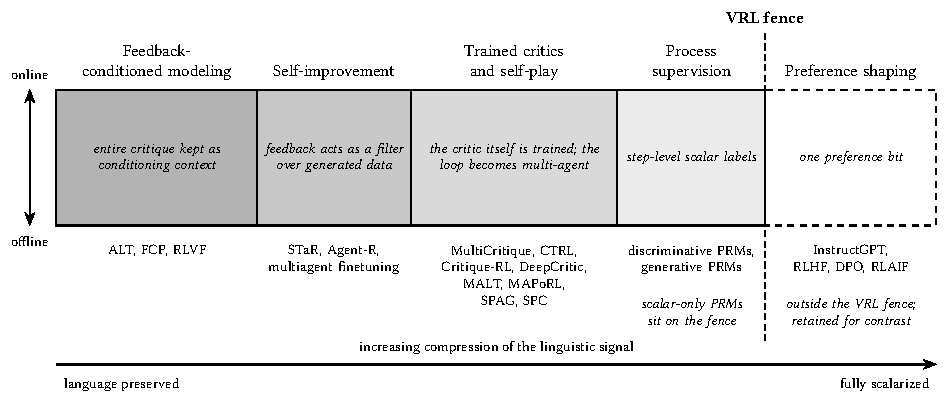
\includegraphics[width=\linewidth]{paper_images/generated/compression_spectrum.pdf}
    \Description{A horizontal spectrum orders feedback-conditioned modeling, self-improvement, trained critics and self-play, process supervision, and preference shaping by increasing compression. A vertical marker shows the VRL fence, and an orthogonal axis distinguishes online from offline feedback.}
    \caption{Training-time methods ordered by how much linguistic structure survives into the parameter update. The dashed fence places scalar-only preference optimization outside VRL and scalar-only process supervision on its boundary. Online and offline collection cut across every band.}
    \label{fig:compression-spectrum}
\end{figure}

\subsection{Feedback-Conditioned Modeling}
\label{subsec:feedback-conditioned}

At the least-compressed end, the learner receives the critique together with the response it should produce. ALT shows why retaining the critique matters, and the feedback-conditional policy formalizes training as maximum likelihood over response-feedback pairs followed by optional online bootstrapping \citep{lloret2024towards,luo2025fcp}. This family preserves corrective detail and supports targeted scope, but it also risks teaching indiscriminate compliance with inaccurate feedback.

\subsection{Self-Improvement}
\label{subsec:self-improvement}

Self-improvement uses language as a filter over model-generated trajectories. STaR retains reasoning paths that reach correct answers, while Constitutional AI filters revisions against written principles \citep{zelikman2022star,bai2022constitutional}. The approach scales cheaply because training consumes ordinary supervised examples. Its bottleneck is filter quality: when the same model generates and judges candidates, systematic errors can compound across rounds.

\subsection{Trained Critics and Critique-Based Fine-Tuning}
\label{subsec:trained-critics}

A trained critic makes feedback production an explicit capability. CTRL optimizes a critic for the downstream correction it induces, while DeepCritic combines deliberate critique with reinforcement learning over step labels \citep{xie2025teaching,yang2025deepcritic}. The design is useful when a frozen general-purpose judge limits improvement, but critic evaluation must separate helpfulness from discriminability. A critic that produces persuasive but poorly localized feedback can improve revisions while remaining an unreliable training signal.

\subsection{Multi-Agent and Self-Play Training}
\label{subsec:selfplay-training}

Jointly training feedback producers and consumers turns the loop into a multi-agent learning problem. MALT propagates outcome credit through generator, verifier, and refiner roles, while MAPoRL co-trains discussion participants for corrective and persuasive contributions \citep{motwani2024malt,park2025maporl}. Self-play can reduce external annotation, but co-adaptation creates its own instability and may reward persuasion rather than truth. The transcript's destination determines placement: context-only debate is deliberative, while transcripts or rewards that alter weights belong here.

\subsection{Process Supervision}
\label{subsec:process-supervision}

Process supervision attaches judgments to intermediate reasoning steps. Scalar click labels alone fail the linguistic-structure criterion, even when one score is provided per step. Generative process reward models remain inside the fence because language is consumed during reward computation, and free-form step critiques qualify when their content determines where credit lands \citep{lightman2024let,zhao2025genprm}. Finer granularity improves localization but raises annotation and verification cost, especially outside mathematics and code.

\subsection{Preference Shaping: The Scalar Endpoint}
\label{subsec:preference-shaping}

Preference shaping collapses a comparative judgment to one bit. InstructGPT established the reward-model plus policy-optimization recipe, and DPO trains directly from preference pairs \citep{ouyang2022training,rafailov2023direct}. These methods are retained as the compression endpoint, not as VRL proper, because the learner never consumes the rationale. Online collection can follow new policy failures; offline objectives inherit the coverage and biases of a fixed corpus.

\paragraph{Synthesis: compression versus optimizability:}
The spectrum is a conditional design rule. Preserve critiques when feedback is trustworthy and a consumer can use their structure; filter generated data when a cheap verifier exists; train critics when feedback production is the bottleneck; use process signals when localization justifies their cost; and scalarize only when throughput matters more than explanatory content. Rich feedback can improve sample efficiency, but stale offline feedback and self-generated judgments introduce coupled bias. The electronic supplement records the secondary systems, algorithmic variants, and benchmark evidence behind each band.

\section{The Verbal Reward Stack}
\label{sec:rewardstack}

The learning-signal pillar (\S\ref{sec:learning}) examined how verbal feedback is compressed into parameter updates. This section asks the prior question: where does the reward itself come from? Training-time VRL has converged on four reward constructions, and we argue they are best read as a single progression: verifiable outcome rewards, rubric rewards, generative reward models, and process reward models (PRMs). Two properties order the rungs. The first is how much linguistic structure participates in computing the reward. The second, which we call the \emph{scalarization boundary}, is the point in that computation at which language collapses into the scalar the optimizer consumes. Ascending the stack moves the boundary later in the pipeline and attaches the signal at finer granularity, at rising verification cost. Table~\ref{tab:rewardstack} summarizes the progression; \S\ref{subsec:scalarization} makes the boundary explicit and traces its consequences.

\begin{table}
\caption{The verbal reward stack. Each rung is characterized by where linguistic structure collapses into the scalar consumed by the optimizer (the scalarization boundary) and by the granularity at which the signal attaches to the trajectory.}
\label{tab:rewardstack}
\small
\begin{tabular}{@{}p{0.14\textwidth}p{0.27\textwidth}p{0.22\textwidth}p{0.1\textwidth}p{0.15\textwidth}@{}}
\toprule
Rung & Reward computation & Scalarization boundary & Granularity & Representative work \\
\midrule
Verifiable outcome & Programmatic check against ground truth & At the environment; no linguistic structure in the reward & Episode & \citep{lambert2024tulu,guo2025deepseek} \\
Rubric reward & Judge checks instance-specific criteria; item scores pooled & At aggregation of criterion verdicts & Response & \citep{gunjal2025rubrics,viswanathan2025checklists,huang2025reinforcement} \\
Generative reward model & Judge writes principles and critique, then a verdict & At verdict emission; critique retained as an audit trail & Response & \citep{zhang2025genrm,liu2025inferencetime,chen2025rmr1} \\
Process reward & Step-level verification, increasingly verbalized & Per step (per token at the limit) & Step or token & \citep{wang2024mathshepherd,khalifa2025processrewardmodelsthink,xu2026rubrics} \\
\bottomrule
\end{tabular}
\end{table}

\subsection{Verifiable Outcome Rewards}
\label{subsec:rlvr}

The bottom rung is reinforcement learning with verifiable rewards (RLVR), a term introduced by the Tulu 3 post-training recipe, which combined supervised fine-tuning, preference optimization, and RL against programmatic correctness checks in a fully open pipeline \citep{lambert2024tulu}. DeepSeek-R1 supplied the flagship result: pure RL against verifiable outcomes, with no human-labeled reasoning trajectories, produced emergent self-reflection and verification behavior and outperformed counterparts trained by supervised learning on human demonstrations across verifiable mathematics, coding, and STEM tasks \citep{guo2025deepseek}. In the vocabulary of \S\ref{sec:framework}, RLVR is the degenerate case of the stack: scalarization happens at the environment itself, and no linguistic structure enters the reward. We include it because it is the baseline every higher rung generalizes, and because its limitations motivated the climb. Verifiable rewards are sparse in agentic settings; Agent-RLVR densifies them with teacher-style verbal guidance, plans and error feedback attached to failed attempts, lifting pass@1 on SWE-Bench Verified from 9.4\% to 22.4\%, and to 27.8\% with a reward model trained on the guided data \citep{da2025agentrlvr}. Verifiable rewards also reach only domains with checkable answers, the gap the rubric rung addresses. Even within their domain, measured gains deserve caution: a position paper on RLVR's hidden costs shows that budget mismatches, attempt inflation with calibration drift, and benchmark contamination confound many headline results, several of which shrink substantially or disappear under budget-matched reproduction \citep{wu2025position}. We revisit this measurement problem in \S\ref{sec:evaluation}; it matters here because every rung above inherits RLVR's optimization machinery, and often its evaluation habits.

\subsection{Rubric Rewards}
\label{subsec:rubrics}

Rubric rewards extend verifiability to open-ended domains by replacing the ground-truth check with instance-specific criteria that a judge evaluates and an aggregation step pools into a scalar. Rubrics as Rewards is the anchor method: scoring rollouts against per-instance rubrics yields relative gains of up to 31\% on HealthBench and 7\% on GPQA-Diamond over LLM-as-judge baselines that assign direct Likert scores, and the structured criteria let smaller judges score more consistently \citep{gunjal2025rubrics}. Checklist feedback makes the same move for instruction following: per-instruction criteria scored by AI judges and verifier programs form an RL reward that is the only method in its comparison to improve on every benchmark, including a four-point gain in hard satisfaction rate on FollowBench \citep{viswanathan2025checklists}.

Rubric supply creates a three-way choice between coverage, adaptation, and verification cost. Large static banks dominate when the task distribution is broad but stable: human and synthetic collections scale open-ended RL, while coarse-to-fine or contrastive generation reduces authoring cost and derives criteria from examples \citep{huang2025reinforcement,li2026rubrichub,liu2025openrubrics}. Dynamic rubrics dominate when the policy or case mix changes during training, because fixed criteria become stale and expose exploitable omissions. Online generation, policy-coupled evolution, self-rewarding, and case-conditioned criteria all trade additional judge calls for criteria matched to the current failure distribution \citep{rezaei2025online,guan2026evorubric,ye2025selfrewarding,wang2025infimedorbit}. Selective verification is preferable when checking every criterion costs more than generating candidates: an adversarial critic can surface only likely violations for external validation and outperform exhaustive checking with fewer verifications \citep{wu2025rlac}. The same logic applies even in domains with correct answers. Process-oriented rubrics catch invalid derivations that outcome checks miss, raising Verified Pass@1024 on AIME2024 from 26.7\% to 62.6\% while reducing ``Miracle Steps'' by 71\% \citep{yuan2025curing}. Static banks therefore buy amortized coverage, dynamic rubrics buy robustness to distribution shift, and selective or process checks buy precision where verification is expensive or outcome correctness is insufficient.

The closest prior survey treats rubrics as a framework recurring across evaluation, RL, and safety, organized into evaluative, training, and intrinsic levels \citep{chen2026from}. Our reading is complementary but different: we place rubrics as one rung of a reward stack ordered by scalarization and granularity, which exposes what they share with the verifiers below and the generative judges above. For this rung, scalarization occurs at aggregation: linguistic structure survives through criterion checking, but once item verdicts are pooled, anything the rubric failed to anticipate is invisible to the training signal, a slack we return to in \S\ref{subsec:scalarization}.

\subsection{Generative Reward Models}
\label{subsec:genrm}

The third rung verbalizes the reward computation itself. Generative verifiers recast reward modeling as next-token prediction: the verifier writes a verification chain of thought before its verdict, inheriting instruction following and majority voting over sampled rationales, and improves best-of-N accuracy from 5\% to 45.3\% on algorithmic tasks and from 73\% to 93.4\% on GSM8K \citep{zhang2025genrm}. DeepSeek-GRM extends this to generalist reward modeling through self-principled critique tuning, online RL that teaches the model to generate principles and then critiques, and shows that sampling more reward computations at inference, guided by a meta reward model, can outperform scaling the reward model's size at training time \citep{liu2025inferencetime}. A growing cluster treats verdict production as a reasoning task in its own right: chain-of-rubrics reward models self-generate rubrics or reference solutions before judging, outperforming far larger open and proprietary models by up to 4.9\% \citep{chen2025rmr1}; reward reasoning models spend adaptive test-time compute on hard judgments \citep{guo2025reward}; J1 converts judgment itself into a verifiable-reward RL problem \citep{whitehouse2025j1}; EvalPlanner decouples evaluation planning from execution, reaching 93.9 on RewardBench \citep{saha2025learning}; and further variants optimize judgment-thinking traces with offline and online RL \citep{huang2025thinkj}, extend judges to long-horizon reasoning \citep{hong2025thinkrm}, or pair a reasoning reward model with a dedicated benchmark (\S\ref{sec:evaluation}) \citep{zhou2025libra}.

Supervision for the judges is increasingly self-generated. Self-taught evaluators iterate without any human preference labels, improving a 70B judge from 75.4 to 88.3 on RewardBench \citep{wang2024selftaught}; jointly predicting critiques and scalar rewards improves reward accuracy by 3.7\%--7.3\% \citep{yu2024selfgenerated}; self-training on unlabeled data yields foundation reward models that emit labels with rationales \citep{wang2025gramr2}; and meta-rewarding has the model judge its own judgments, the recursive rung of the stack, lifting the AlpacaEval~2 win rate from 22.9\% to 39.4\% \citep{wu2024metarewarding}. The critique, however, is not automatically load-bearing: generative reward models trained only on verdict correctness learn to guess right outcomes from unsound critiques, and supervising the critique itself, by rewarding similarity to human critiques, outperforms outcome-only training \citep{wang2026reward}, closing the loop between the reward layer and the human verbal feedback of \S\ref{sec:learning}. For this rung, scalarization occurs at verdict emission: the verbal computation demonstrably improves the verdict and leaves an auditable trail, but the optimizer still consumes a scalar unless the critique is separately routed into revision or a language-space update (\S\ref{sec:optimizers}).

\subsection{Process Reward Models}
\label{subsec:prm}

The fourth rung moves the signal inside the trajectory. PRMs descend from human step-level annotation \citep{lightman2024let}, which automation quickly replaced: Math-Shepherd constructs step labels automatically and lifts GSM8K accuracy from 77.9\% to 84.1\% through step-by-step PPO \citep{wang2024mathshepherd}, and OmegaPRM's divide-and-conquer tree search locates the first error by binary search, collecting over 1.5 million step annotations and improving MATH500 from 51\% to 69.4\% with weighted self-consistency \citep{luo2024improve}. The subsequent diagnosis was sobering. ProcessBench, an error-localization benchmark whose protocol \S\ref{sec:evaluation} describes, finds that existing PRMs typically fail to generalize beyond GSM8K/MATH difficulty and underperform prompted critic models \citep{zheng2024processbench}. A companion study explains why: Monte Carlo-estimated step labels underperform LLM-as-a-judge and human annotation because completion models verify steps inaccurately, and best-of-N evaluation quietly drifts PRMs back toward outcome scoring; consensus filtering between the two estimators significantly improves performance and data efficiency \citep{zhang2025lessons}.

Generative PRMs are where the judge line and the step line converge. ThinkPRM verifies every step by generating a verification chain of thought, outperforming discriminative verifiers with only 1\% of the PRM800K labels \citep{khalifa2025processrewardmodelsthink}; StepWiser reframes stepwise reward modeling from classification to reasoning, training the judge with RL from rollout outcomes \citep{xiong2025stepwiser}; and DG-PRM maintains a tree of fine-grained reward criteria selected dynamically per step \citep{yin2025dynamic}. SPARK closes the loop for domains without verifiable answers: synthetic step-level verification data trains a PRM that then drives RL, beating ground-truth RLVR at 47.4\% versus 43.9\% averaged over six mathematics benchmarks \citep{rahman2025spark}, and OmegaPRM-style pipelines now extend to multimodal reasoning with over 700k automatically generated step annotations \citep{du2025mmprm}. At the finest granularity, response-level rubrics can be converted into token-level credit through a relevance discriminator \citep{xu2026rubrics}, at which point the reward stack meets the credit-assignment problem of \S\ref{sec:credit}.

\subsection{The Scalarization Boundary}
\label{subsec:scalarization}

We can now state the section's organizing claim plainly. Every rung ends the same way: a scalar crosses the interface to the optimizer. What distinguishes the rungs is where the collapse happens. Verifiers scalarize at the environment; rubrics at aggregation, after criterion-level checking; generative reward models at verdict emission, after a full verbal computation; PRMs per step; token-level methods per token. What is lost at the boundary is everything the verbal computation established that a magnitude cannot carry: which failure occurred, what would repair it, and why the trajectory earned its score. The gradient sees that a rollout scored 0.3, not that it scored 0.3 because its third step asserted an unsupported lemma. Ascending the stack narrows the loss by shrinking the span each scalar summarizes, but only the language-space optimizers of \S\ref{sec:optimizers} remove the boundary altogether, applying feedback as text without collapsing it. In the terms of \S\ref{sec:framework}, rubric scores and PRM verdicts are verbal reward functions, language occupying the role of the reward function in the underlying decision process; the practitioner question of which rung to adopt, a tradeoff between signal granularity and verification cost, is taken up in \S\ref{sec:practitioner}.

The boundary is also where reward hacking concentrates, because whatever the verbal computation understood but the scalar cannot transmit becomes exploitable slack. The evidence spans every rung. Outcome rewards breed Miracle Steps \citep{yuan2025curing}, and static rubrics are gameable by design \citep{rezaei2025online}. A systematic study of rubric-based RL locates the exploitation in precisely this slack: when rubrics leave failure modes unspecified, rubric-based verifiers prefer the trained checkpoint while rubric-free judges prefer the base model \citep{mahmoud2026reward}, a finding set \S\ref{sec:safety} examines in full. One rung up, generative reward models guess correct verdicts from unsound critiques \citep{wang2026reward}; one rung further, mis-estimated step labels corrupt PRM training \citep{zhang2025lessons}; and at the base, headline RLVR gains partly dissolve under budget-matched evaluation \citep{wu2025position}. The emerging defenses sit, tellingly, at the boundary itself: cross-family judge panels with a verifier-free self-internalization diagnostic \citep{mahmoud2026reward}, meta-verification and peer consensus over self-generated rubrics \citep{guan2026evorubric}, format constraints on PRM-driven RL \citep{rahman2025spark}, and consensus filtering of step labels \citep{zhang2025lessons}. Whether these patches suffice, or whether the boundary itself must move, is the safety question of \S\ref{sec:safety}.

\section{Credit Assignment and Optimization with Verbal Signals}
\label{sec:credit}

Credit assignment asks which parts of an agent's behavior deserve blame or praise for a delayed outcome. Language makes this problem harder because an LLM action may span thousands of tokens and several turns, yet it also offers a distinctive solution: a critique can name the faulty step and the needed repair, information that no scalar carries. We organize the literature by the granularity at which credit lands (outcome, step, turn, token, or memory operation) and by its carrier (redistributed scalar, model-internal attribution, or critique text). These choices determine which optimizer can consume the signal and which assumptions must hold.

\begin{table}[t]
\centering
\caption{Families of credit-assignment mechanisms in VRL, ordered by how much linguistic content the credit carrier consumes.}
\label{tab:credit-families}
\small
\begin{tabular}{@{}p{0.19\textwidth}p{0.30\textwidth}p{0.13\textwidth}p{0.26\textwidth}@{}}
\toprule
Family & Credit carrier & Granularity & Representative work \\
\midrule
Temporal abstraction & scalar reward over macro actions or turns & span, turn & \citep{chai2024marlhf,zhou2024archer,wei2025reinforcing} \\
Reward redistribution & holistic scalar re-allocated after the fact & token or time step & \citep{li2024red,qu2024latent} \\
Model-internal attribution & explainability scores or attention flow & token & \citep{koo2025learning,dong2026how} \\
Information-theoretic & belief update about the final answer & turn & \citep{wang2025information} \\
Generative process critique & step-wise critique converted to credit & step, token & \citep{xie2025capo,zhou2024treg,wang2026text2gradreinforcementlearningnatural,liu2025agenticreinforcementlearningimplicit} \\
LLM-as-annotator & subgoal and action judgments by an external LLM & action, subgoal & \citep{pignatelli2024assessing,zhong2024policy,lin2025speaking} \\
Memory-conditioned & credit assigned to memory operations & memory write & \citep{zhou2025memento,yan2026memoryr2} \\
\bottomrule
\end{tabular}
\end{table}

\subsection{Outcome, Process, and Reflective Credit}
\label{subsec:credit-granularity}

Three levels recur. \emph{Outcome credit} scores only the final trajectory. It is cheap and exact for verifiable tasks, which makes it suitable for group-comparison methods, but broadcasting one scalar over every token is maximally coarse \citep{guo2025deepseek}. \emph{Process credit} judges intermediate steps; process supervision and process reward models make a delayed outcome locally actionable \citep{uesato2022solving,lightman2024let}. \emph{Reflective credit} uses the content of an evaluation $\ell$, rather than only its scalarization $\sigma(\ell)$, to determine where and how an update lands. Stored reflections steer later attempts, critiques can be aligned to the spans they indict, and feedback-conditioned policies can retain text as a conditioning variable instead of compressing it \citep{shinn2023reflexion,wang2026text2gradreinforcementlearningnatural,luo2025fcp}. Outcome credit ranks trajectories, process credit ranks steps, and reflective credit can state what to change.

\subsection{Mechanisms and Selection Rules}
\label{subsec:credit-token}

Four mechanisms push sparse outcomes toward the responsible behavior. Temporal abstraction shortens the horizon by treating token spans or turns as macro actions \citep{chai2024marlhf,zhou2024archer}. Reward redistribution preserves a trusted sequence-level scorer but reallocates its value across tokens or time steps \citep{li2024red,qu2024latent}. Model-internal attribution derives token importance from additive explanations or information flow, which makes the shaping signal inspectable but ties it to the reward model's internals \citep{koo2025learning,dong2026how}. Critique-derived methods generate stepwise diagnoses and convert them into token or step credit, gaining semantic localization without a separately labeled dense reward model \citep{xie2025capo,zhou2024treg,liu2025agenticreinforcementlearningimplicit}.

The choice follows the artifacts available before training. Temporal abstraction is the cheapest first move when a trusted outcome reward exists. Redistribution is appropriate when the reward model is the only trusted component; attribution is preferable when the credit trace must be inspected. Critique-derived credit is the only family that can both localize and name an error, but it is justified only when critic quality can be audited. LLM annotation extends the same idea to non-language policies by judging subgoals, transitions, or team contributions, moving the principal failure risk into the annotator \citep{pignatelli2024assessing,zhong2024policy,lin2025speaking}.

\subsection{Long Horizons and Memory}
\label{subsec:credit-multiturn}

Multi-turn interaction introduces two nested questions: which turn helped, and which tokens within it. Hierarchical learners combine turn-level values with within-turn policy gradients; explicit turn rewards are lighter when intermediate outcomes are checkable; information-gain rewards use the policy's belief update when no external reward model is available \citep{zhou2024archer,wei2025reinforcing,wang2025information}. Persistent memory adds a state-conditioned credit problem. Because memory writes change the effective environment seen by later rollouts, group-relative comparisons become biased unless memory operations are compared from a shared intermediate state \citep{zhou2025memento,yan2026memoryr2}. Turn-level rewards are therefore an optional refinement, but memory-conditioned credit is mandatory once the agent writes persistent state.

\subsection{Optimizer Pairing}
\label{subsec:credit-algorithms}

Feedback form constrains the optimizer. Executable rewards pair naturally with online policy gradients; pairwise judgments with offline preference objectives; filtered or feedback-conditioned text with supervised fine-tuning; and step-level judgments with process reward models \citep{schulman2017proximal,rafailov2023direct,luo2025fcp,lightman2024let}. Group comparison adds an assumption that rollouts share an environment and reward scale, which turn structure and memory writes can violate \citep{guo2025deepseek,wei2025reinforcing,yan2026memoryr2}. Language-mediated states also risk information loss, and language-generated actions alter exploration. Planner-imitated subgoals, for example, require explicit exploration to avoid linear regret \citep{he2024words}. The practitioner should therefore choose the feedback carrier first and treat the optimizer as a downstream consequence.

\subsection{The State of Theory}
\label{subsec:credit-theory}

General theory remains thin. The main formal anchor is learning from language feedback through transfer eluder dimension \citep{xu2025formalizing}. Partial results cover regret for language-mediated hierarchies, optimality preservation under feature-additive shaping, redundancy reduction for latent rewards, and the derivation of implicit step rewards \citep{he2024words,koo2025learning,qu2024latent,liu2025agenticreinforcementlearningimplicit}. Missing are conditions under which critique-derived token credit preserves the optimal outcome policy and bounds on how verbal localization errors compound through training. This gap is central to the research agenda in \S\ref{sec:practitioner}.

\section{Language-Space Optimizers}
\label{sec:optimizers}

The improvement operator of \S\ref{sec:framework} can revise one output, write persistent memory, or update model parameters. Language-space optimization occupies the middle ground: an outer optimizer treats a prompt, context, playbook, or scaffold as an editable system parameter and improves it against a task metric. It is therefore not a fourth pillar. The optimized text persists across episodes like a learning artifact, but a frozen model consumes it through the context window. This semi-parametric view also clarifies the analogy to numerical optimization: critique supplies directional information, text is the parameter, an LLM edit is the update, and execution traces route credit through compound systems \citep{xiao2024verbalized,cheng2024trace}.

\subsection{Mechanism Families}
\label{subsec:optimizers-search}

Four families differ in the information supplied to the update. \emph{Score-driven search} proposes candidates and retains those with higher task scores; OPRO places previous candidates and scores in context so the optimizer can exploit its search history \citep{yang2024opro}. \emph{Textual-gradient methods} replace a scalar score with a diagnosis and propagate it to the responsible prompt or program component; TextGrad is the canonical realization, while trace-based methods extend the idea to compound graphs \citep{yuksekgonul2024textgrad}. \emph{Reflective and evolutionary methods} maintain diverse candidates, diagnose failures, and select complementary improvements; GEPA shows that richer diagnoses can achieve stronger sample efficiency than policy-gradient updates when rollouts are scarce \citep{agrawal2026gepa}. \emph{Hybrid methods} alternate text edits with weight updates, using prompt evolution to escape failures and then distilling the gain into the model; P$^2$O exemplifies this division of labor \citep{lu2026p2o}. Detailed systems and quantitative comparisons appear in the electronic supplement.

The families also assign credit at different resolutions. Score-only search credits a whole candidate, which is simple but expensive when pipelines contain many coupled prompts. Textual gradients use execution traces to localize blame to a component. Reflective populations trade precise attribution for diversity, retaining several explanations or solutions when no single update dominates every objective. Hybrids add a second choice: whether a discovered improvement should remain explicit in context or become procedural knowledge in weights. This credit unit, candidate, component, population, or parameter update, is often more consequential than the particular LLM used as optimizer.

\subsection{Selection Rules and Failure Modes}
\label{subsec:optimizers-tradeoffs}

Language-space optimization is preferred when weights or gradients are inaccessible, supervision is scarce enough that explanatory feedback must extract more information per rollout, or the learned artifact must remain inspectable and editable. Trace-aware textual gradients are especially useful when a compound pipeline needs component-level credit. Population methods help when several objectives or qualitatively different solutions must be retained. Weight updates remain preferable when abundant data amortizes training, the target knowledge is procedural, or deployment cannot afford a growing context. Hybrid methods fit the intermediate case, where an interpretable prompt discovers a behavior that must later be internalized.

The same properties create predictable failures. A reflective optimizer can misdiagnose the cause of an error and move in the wrong direction \citep{ma2024are}; wholesale context rewriting can collapse useful detail \citep{zhang2025agentic}; multi-objective critiques can dilute task focus \citep{darshan2026when}; and poisoned feedback directly poisons the update channel. Two contrast cases mark the definitional fence: text optimized by actual numeric gradients or by selection signals with no linguistic meaning is prompt optimization, but not verbal reinforcement learning \citep{das2024greater,wang2025evolving}. The verbal channel primarily buys sample efficiency, auditability, and an interface for structured credit, not a guarantee of higher attainable performance.

\section{Language Feedback in Embodied and Multimodal Settings}
\label{sec:embodied}
% BRIEF (new; T6 notes; fixes weakness (h)): feedback is natural language, observations
% are non-text. Language corrections to robot policies (YAY Robot, DROC, LILAC, RT-H),
% language-to-reward (Eureka, L2R, Text2Reward, DrEureka), VLM reward models (RoboReward,
% Robo-Dopamine), failure reasoning (AHA). Scope statement mirrors S2 fence.
\todonote{Draft from T6 notes.}

\section{Evaluation and Benchmarks}
\label{sec:evaluation}

Evaluation must separate feedback \emph{quality}, whether a signal is accurate, calibrated, and unbiased, from feedback \emph{utilization}, whether the receiving system improves when that signal is supplied. The axes are independent: a correct critique can be ignored, while a reward model can score well on held-out preferences yet train a worse policy \citep{kim2024evaluating}. Treating end-task accuracy as a single summary obscures whether failure lies in the signal, the receiver, or their interface.

\subsection{Measuring Feedback Quality}
\label{subsec:eval-quality}

Quality benchmarks should match the signal's granularity and operational role. Outcome-preference benchmarks test reward-model ranking; RewardBench~2 is an anchor because it validates benchmark scores against best-of-$N$ selection and PPO outcomes rather than assuming pairwise accuracy transfers \citep{malik2025rewardbench}. Judge meta-evaluation tests verdict consistency and bias; JudgeBench ties labels to objective correctness and finds even strong judges only slightly above chance on hard pairs \citep{tan2024judgebench}. Critique benchmarks score error identification and correction; CriticBench evaluates generation, critique, and repair jointly \citep{lin2024criticbench}. Process benchmarks localize step-level errors; ProcessBench asks for the first erroneous reasoning step, directly testing the signal consumed by process supervision \citep{zheng2024processbench}. Embodied instruments test whether vision-language judges understand trajectories rather than final frames; ViSTa exposes severe weakness on sequential tasks \citep{wybitul2024vista}. These families are not interchangeable: a judge validated for reranking is not automatically a sound training reward or a useful critic.

Validity requires more than difficulty. Pairwise accuracy should predict the downstream use, and test distributions should expose length, style, refusal, and format. Process evaluation must separate error localization from final verdict because a wrong location misassigns credit. Generative critiques should separate factual correctness from actionable specificity. Report uncertainty and judge disagreement when small differences determine system selection.

\subsection{Measuring Feedback Utilization}
\label{subsec:eval-utilization}

Utilization benchmarks score the receiver under a controlled signal. RealCritic measures a critique through the correction it induces and shows that plausible open-loop critiques can fail to improve self-revision \citep{tang2025realcritic}. Interactive environments isolate feedback uptake across attempts; LLF-Bench uses post-action language as the learning signal and paraphrases feedback to prevent task recognition from masquerading as learning \citep{cheng2023llfbench}. Feedback Friction supplies near-oracle feedback yet finds that solvers still resist incorporating it, demonstrating that utilization can remain the bottleneck after quality is nearly solved \citep{jiang2025feedback}. Long-horizon settings add retrieval and temporal credit: MemoryAgentBench tests whether accumulated verbal experience is retrieved, used, and selectively forgotten across episodes \citep{hu2025evaluating}. The detailed benchmark matrix and evidence catalog are provided in the electronic supplement.

A clean utilization study varies the signal while holding task, receiver, and budget fixed. A no-feedback control measures prior capability; an oracle condition estimates attainable gain; irrelevant feedback tests resistance to persuasive noise. Report improvement per interaction or token, and test several receivers because one critique can help a capable model yet overwhelm a weaker one.

\subsection{Measurement Gaps and Minimum Reporting Protocol}
\label{subsec:eval-gaps}

Current evidence is strongest for short, verifiable, English, single-turn tasks and weakest for personalized, multilingual, long-horizon, adversarial, and embodied feedback. Judge-scored results inherit the judge's consistency, bias, and aggregation uncertainty. Embodied benchmarks largely grade signal quality and rarely test whether a motor policy can use verbal feedback. Static evaluation also misses failures that emerge only when outputs change later observations or rewards.

These gaps limit claims of generality. Results from a short answer verifier do not establish trajectory-level credit, and an English critique benchmark does not establish that the same feedback interface transfers across languages or cultures. Evaluation should therefore state the intended deployment regime and treat movement beyond the benchmark's signal type, horizon, modality, or interaction structure as an explicit extrapolation.

A minimum reporting protocol follows. (1)~Report feedback quality and utilization separately. (2)~Validate a quality benchmark against its downstream use, such as best-of-$N$ selection, policy optimization, correction success, or task completion. (3)~Audit judges and verifiers for consistency, bias, and adversarial robustness before using their verdicts as evaluation or reward. (4)~State the signal type, granularity, interaction stage, and receiver, so results transfer only to mechanisms with the same role. When possible, include a no-feedback control and an oracle-feedback upper bound; their gap separates absent information from failed uptake. This protocol does not yet solve the lack of standardized utilization metrics, but it prevents quality and utilization failures from being conflated.

\section{Safety and Robustness of Feedback Channels}
\label{sec:safety}
% BRIEF (new differentiator; T8 notes): attacks on the feedback channel itself.
% Judge injection (JudgeDeceiver, one-token RLVR fooling), agent injection (AgentDojo,
% InjecAgent, WASP), poisoned optimizer feedback (attacks the S9 loop), rubric reward
% hacking (CHERRL, hack-verifiable environments), sycophancy as corrupted feedback
% (SycEval, SYCON-Bench, ELEPHANT), in-context reward hacking feedback loops. Defenses:
% instruction hierarchies, adversarial fine-tuning, provenance. Expands the ACL 6.3 cell.
\todonote{Draft from T8 notes.}

\section{Practitioner Guide, Related Surveys, and Research Agenda}
\label{sec:practitioner}

The preceding sections classify the literature; this section turns the classification outward. We first distill the taxonomy of \S\ref{sec:taxonomy} into prescriptive guidance for choosing a verbal-feedback mechanism (\S\ref{subsec:mechanism}), then position the survey against eighteen prior surveys and frameworks (\S\ref{subsec:priorsurveys}), and close with a ten-item research agenda assembled from the gaps named in \S\ref{sec:framework} through \S\ref{sec:safety} (\S\ref{subsec:agenda}).

\subsection{Choosing a Verbal-Feedback Mechanism}
\label{subsec:mechanism}

Table~\ref{tab:practitioner} states when each role for language is the right choice, keyed to properties a practitioner can assess before building anything: whether task outcomes are mechanically verifiable, whether model weights are accessible, the latency and cost budget available for producing feedback, and the dominant risk that must be monitored once the mechanism is in place. The six rows correspond to the placements developed in \S\ref{sec:grounding} through \S\ref{sec:rewardstack}; representative methods are drawn from the sections where each mechanism is analyzed.

\begin{table}[t]
    \centering
    \footnotesize
    \renewcommand{\arraystretch}{1.2}
    \caption{Practitioner guidance: when to use language in each role, what it costs, and what to monitor.}
    \label{tab:practitioner}
    \begin{tabularx}{\textwidth}{@{} >{\raggedright\arraybackslash}p{0.13\textwidth} >{\raggedright\arraybackslash}X >{\raggedright\arraybackslash}p{0.155\textwidth} >{\raggedright\arraybackslash}p{0.15\textwidth} >{\raggedright\arraybackslash}p{0.17\textwidth} @{}}
        \toprule
        \textbf{Language as} & \textbf{Preconditions} & \textbf{Latency and cost} & \textbf{Dominant risk} & \textbf{Representative} \\
        \midrule
        Reward (compiled to code or rubric) & Success expressible as checks; simulator or executor available; weights and training budget accessible & Offline compilation; cheap per episode once compiled & Objective mis-specification; reward hacking & Eureka \citep{ma2024eureka}; Text2Reward \citep{xie2024text2reward} \\
        State or task grounding & Raw observations too complex or task underspecified; language abstracts them faithfully & Per-step description cost; no training required & Information loss; state aliasing & ALFWorld \citep{shridhar2020alfworld}; SayCan \citep{ahn2022can} \\
        Action guidance & Open-ended action space; LLM priors informative; actions executable and checkable & Per-step generation cost & Exploration collapse under the prior; unexecutable actions & ReAct \citep{yao2023react}; ProgPrompt \citep{singh2022progprompt}; CodeAct \citep{wang2024executable} \\
        Deliberative feedback & No weight access; latency budget allows iteration; a grounded critic (tools, tests) exists & Multiplies inference cost per query & Circular self-critique; unbounded revision loops & Self-Refine \citep{madaan2023selfrefine}; CRITIC \citep{gou2024critic}; ToT \citep{yao2023tree} \\
        Memory & Tasks recur across episodes; lessons are reusable & Cheap writes; retrieval overhead per episode & Error persistence; memory poisoning & Reflexion \citep{shinn2023reflexion}; ExpeL \citep{zhao2024expel}; Voyager \citep{wang2023voyager} \\
        Training signal & Persistent improvement needed; feedback plentiful; weights accessible & Highest upfront cost; amortizes across deployment & Sycophancy to wrong critiques; filter bias & FCP \citep{luo2025fcp}; STaR \citep{zelikman2022star}; generative PRMs \citep{zhao2025genprm} \\
        \bottomrule
    \end{tabularx}
\end{table}

The choice of mechanism also constrains the choice of optimizer: each feedback form pairs with a particular optimization family, and each pairing imports its own assumptions into the decision problem, as analyzed in \S\ref{sec:credit}. The guidance below therefore fixes the feedback form first and treats the optimizer as a downstream consequence of that choice.

The table compresses into four ordered questions. First, are model weights accessible? If so, a second question selects the training signal: when the outcome is mechanically verifiable, compile the language into an executable reward or rubric and train against it (\S\ref{sec:rewardstack}), after which the monitoring burden shifts to hacking of the compiled objective; when it is not but verbal feedback is plentiful, train on that feedback directly through feedback-conditioned methods such as FCP \citep{luo2025fcp}, monitoring for sycophancy and filter bias (\S\ref{sec:learning}). Third, if weights are inaccessible but the latency budget allows iteration, use deliberative feedback, and prefer a critic grounded in tools or tests over prompted self-critique, which does not succeed without reliable external signal \citep{kamoi2024can,gou2024critic}. Fourth, if the latency budget does not allow iteration but tasks recur across episodes, persist distilled lessons as memory and audit the store for stale or poisoned entries (\S\ref{sec:safety}). When every branch fails its preconditions (nothing verifiable to compile, no plentiful feedback to train on, no latency budget for iteration, no recurring tasks), the bottleneck is specification rather than optimization: spend the language budget on grounding, describing states, defining the task, or constraining actions before any feedback loop is built. Figure~\ref{fig:decision-tree} arranges the four questions as a decision tree.

\begin{figure}[t]
    \centering
    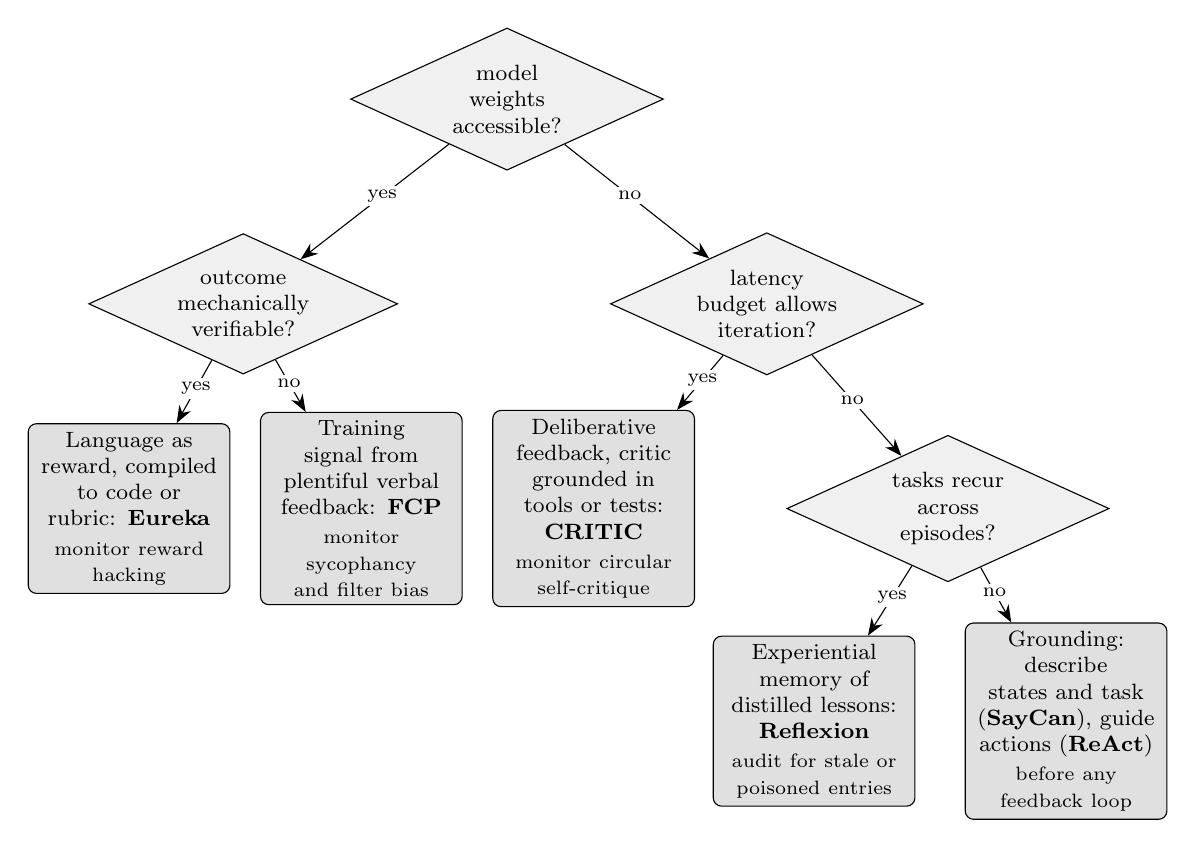
\begin{tikzpicture}[
        font=\footnotesize,
        >={Stealth[length=2.2mm]},
        every node/.append style={execute at begin node={\hyphenpenalty=10000\exhyphenpenalty=10000\relax}},
        decision/.style={diamond, aspect=2.2, draw, align=center,
            inner sep=1pt, text width=1.85cm, fill=black!6},
        leaf/.style={rectangle, rounded corners=3pt, draw, align=center,
            inner sep=3pt, text width=2.35cm, fill=black!12},
        ans/.style={font=\scriptsize, fill=white, inner sep=1.5pt}
    ]
        \node[decision] (d1) at (6.2,0)      {model weights accessible?};
        \node[decision] (d2) at (2.85,-2.6)  {outcome mechanically verifiable?};
        \node[decision] (d3) at (9.5,-2.6)   {latency budget allows iteration?};
        \node[decision] (d4) at (11.8,-5.2)  {tasks recur across episodes?};

        \node[leaf] (l1) at (1.4,-5.2)  {Language as reward, compiled to code or rubric: \textbf{Eureka}\\[1pt]{\scriptsize monitor reward hacking}};
        \node[leaf] (l2) at (4.35,-5.2) {Training signal from plentiful verbal feedback: \textbf{FCP}\\[1pt]{\scriptsize monitor sycophancy and filter bias}};
        \node[leaf] (l3) at (7.3,-5.2)  {Deliberative feedback, critic grounded in tools or tests: \textbf{CRITIC}\\[1pt]{\scriptsize monitor circular self-critique}};
        \node[leaf] (l4) at (10.1,-7.9) {Experiential memory of distilled lessons: \textbf{Reflexion}\\[1pt]{\scriptsize audit for stale or poisoned entries}};
        \node[leaf] (l5) at (13.3,-7.9) {Grounding: describe states and task (\textbf{SayCan}), guide actions (\textbf{ReAct})\\[1pt]{\scriptsize before any feedback loop}};

        \draw[->] (d1) -- node[ans, pos=0.45] {yes} (d2);
        \draw[->] (d1) -- node[ans, pos=0.45] {no}  (d3);
        \draw[->] (d2) -- node[ans, pos=0.45] {yes} (l1);
        \draw[->] (d2) -- node[ans, pos=0.45] {no}  (l2);
        \draw[->] (d3) -- node[ans, pos=0.45] {yes} (l3);
        \draw[->] (d3) -- node[ans, pos=0.45] {no}  (d4);
        \draw[->] (d4) -- node[ans, pos=0.45] {yes} (l4);
        \draw[->] (d4) -- node[ans, pos=0.45] {no}  (l5);
    \end{tikzpicture}
    \caption{Choosing a verbal-feedback mechanism: the four ordered questions of \S\ref{subsec:mechanism} arranged as a decision tree. Each leaf names a row of Table~\ref{tab:practitioner} with one representative method and inherits that row's full preconditions, which the tree does not re-check; the final leaf covers the two grounding roles.}
    \label{fig:decision-tree}
\end{figure}

\subsection{Comparison with Prior Surveys}
\label{subsec:priorsurveys}

To our knowledge, this survey is the first organized around the verbal signal itself: which component of the decision problem a linguistic artifact modifies and when it takes effect. Table~\ref{tab:surveys} makes the positioning explicit against eighteen prior surveys and frameworks. Most shelf neighbors organize by mechanism (correction timing, evolution phase, rollout stage), by agent component (memory, capability, module under optimization), or by algorithm family (RLHF, preference optimization, agentic RL); the nearest exception, the feedback typing of \citet{fernandes2023bridging}, does take the signal as its axis but predates the agentic signals surveyed here. None combines a signal-centric axis with a formal framework, coverage of all three stages (problem definition, inference, and training), and treatment of the feedback channel's safety; that fourfold combination is the position this survey occupies.

\begin{table}[t]
    \centering
    \footnotesize
    \renewcommand{\arraystretch}{1.15}
    \caption{Positioning against prior surveys and frameworks. Feedback types: S = scalar, P = preference, V = verbal; a letter in parentheses marks a feedback type the work treats only partially. Stages: D = problem definition and grounding, I = inference, T = training. Formal (formal framework), Guide (prescriptive practitioner guidance), and Safety (feedback-channel safety): Y = yes, P = partial, N = not claimed. All cells are graded from each work's abstract and stated contributions, so N records the absence of a claim there, not a judgment of the work's full text.}
    \label{tab:surveys}
    \begin{tabularx}{\textwidth}{@{} l >{\raggedright\arraybackslash}p{0.14\textwidth} >{\raggedright\arraybackslash}X >{\raggedright\arraybackslash}p{0.075\textwidth} p{0.05\textwidth} c c c @{}}
        \toprule
        \textbf{Survey} & \textbf{Scope} & \textbf{Organizing axis} & \textbf{Feedb.} & \textbf{Stages} & \textbf{Formal} & \textbf{Guide} & \textbf{Safety} \\
        \midrule
        \citet{luketina2019survey} & language-informed RL (pre-LLM) & task setting & S & T & N & N & N \\
        \citet{pan2023automatically} & LLM self-correction & correction timing & V, (S) & I, T & N & P & N \\
        \citet{kamoi2024can} & self-correction critique & research question $\times$ feedback source & V & I, T & N & Y & N \\
        \citet{fernandes2023bridging} & feedback for generation & format $\times$ objective $\times$ use & S, P, V & I, T & Y & P & P \\
        \citet{wang2024reinforcement} & RL-enhanced LLMs & training technique (RLHF, RLAIF, DPO) & S, P & T & N & P & N \\
        \citet{xiao2024comprehensive} & preference optimization & research questions & P & T & P & P & N \\
        \citet{zhang2025survey} & agent memory & design, evaluation, application & (V) & I & P & P & N \\
        \citet{zhang2025testtime} & test-time scaling & what/how/where/how well & (S), (V) & I & P & Y & N \\
        \citet{gao2025survey} & self-evolving agents & what/when/how to evolve & S, V & I, T & P & P & Y \\
        \citet{fang2025comprehensive} & self-evolving agents & component under optimization & (S), (V) & I, T & Y & P & Y \\
        \citet{du2025survey} & LLM-agent optimization & parameter-driven vs.\ parameter-free & S, (V) & I, T & N & P & N \\
        \citet{zhang2025landscape} & agentic RL & capability $\times$ domain & S, (P) & T & Y & P & N \\
        \citet{srivastava2025technical} & RL for LLMs & reward $\times$ feedback $\times$ optimization & S, P, (V) & T & Y & Y & P \\
        \citet{zhang2026reasoning} & LLM-RL credit assignment & granularity $\times$ methodology & S & T & N & Y & N \\
        \citet{ji2025survey} & alignment & reward-mechanism dimensions & S, P & T & Y & Y & N \\
        \citet{wu2025sailing} & learning from rewards & reward model $\times$ strategy $\times$ stage & S, P, (V) & I, T & N & P & N \\
        \citet{surana2026generate} & RL rollout design & rollout stage & S, (V) & T & Y & Y & P \\
        \citet{feng2024natural} & NLRL (framework) & RL-component analogues in language & V & I, T & Y & N & N \\
        \midrule
        This survey & verbal RL & the signal: what it modifies, when it acts & V, (S), (P) & D, I, T & Y & Y & Y \\
        \bottomrule
    \end{tabularx}
\end{table}

Two rows anchor the history of the idea. \citet{luketina2019survey} argued in 2019 that language should inform a scalar-reward learner; the era surveyed here inverts that premise, since language is now simultaneously the policy medium, the feedback, and increasingly the optimizer trace (\S\ref{sec:optimizers}). Natural language reinforcement learning \citep{feng2024natural} is the closest formal neighbor, but it is one value-centric instantiation, extending RL components into language space, whereas our framework in \S\ref{sec:framework} types the full range of signals and maps the empirical field that the formalism alone does not cover. This positioning also resolves the terminological collision noted in \S\ref{sec:intro}: the coinage of verbal reinforcement learning for self-reflective agents \citep{shinn2023reflexion} names the inference-stage cell of our taxonomy, natural language reinforcement learning names a training-stage formal instantiation, and this survey supplies the signal-centric umbrella over both.

A second cluster fixes the feedback signal in advance and organizes by mechanism. \citet{pan2023automatically} taxonomize by when correction happens; in our terms, correction is one consumption pattern, and we follow the same signals into grounding and the trained reward stack. \citet{kamoi2024can} contribute the field's sharpest negative result, that prompted self-feedback alone does not produce successful self-correction; in our frame this becomes a statement about signal provenance that generalizes across all three pillars. \citet{zhang2025testtime} treat feedback as an implementation detail of scaling, whereas we make the signal the object of study and connect the same signal to training-time consumption. \citet{fernandes2023bridging} offer the closest prior signal typing, a formalization of feedback by format, objective, and use, but it predates agents, verifiable-reward training, rubric rewards, and experiential memory; we extend the typing to agentic settings and to adversarially supplied feedback.

A third cluster organizes by agent component. \citet{zhang2025survey} survey memory as a module; we treat persisted verbal experience as a learning signal governed by an explicit boundary rule (\S\ref{sec:taxonomy}). The two self-evolution surveys \citep{gao2025survey,fang2025comprehensive} classify by which component evolves; we classify by the signal that drives evolution and supply the decision rules for signal choice that a component axis leaves unaddressed. \citet{du2025survey}, an agent survey published in this journal, split optimization at the top level into parameter-driven and parameter-free families, an axis keyed to where an update lands (weights or context); our signal-centric axis unifies those branches, since the same critique can drive a fine-tuning run or a prompt revision. \citet{zhang2025landscape} formalize agentic RL as a shift from single-step to temporally extended decision problems, but their capability-by-domain taxonomy leaves the verbal channel implicit, and their training-centric frame underplays the problem-definition and inference stages we cover.

The final cluster is reward-centric. \citet{wang2024reinforcement} and \citet{xiao2024comprehensive} survey pipelines in which feedback is scalarized into preferences before optimization; our \S\ref{sec:learning} examines precisely what that scalarization discards, namely the verbal rationale attached to a preference and the conditions under which retaining it pays. \citet{srivastava2025technical} bring algorithmic failure-mode depth to RL for LLMs, yet their taxonomy also scalarizes feedback before analyzing it, whereas we keep the language structure of the signal and analyze credit assignment on it directly (\S\ref{sec:credit}). \citet{ji2025survey} read alignment progress as reward-design refinement, assuming the signal must become a reward; we ask when language should remain language. \citet{wu2025sailing} span training, inference, and post-inference stages but from a reward-model-centric view that excludes problem-definition grounding and non-scalarized signals. \citet{surana2026generate} locate where signals enter the rollout pipeline; we specify the semantics of those signals and cover the stages outside the training pipeline entirely. \citet{zhang2026reasoning} go deepest on a single shelf, surveying 47 credit-assignment methods for LLM reinforcement learning in a granularity-by-methodology grid, and contribute a method-selection decision tree of their own; their tree chooses among credit-assignment schemes once training is already the committed mechanism, whereas Figure~\ref{fig:decision-tree} operates one level earlier, selecting which feedback mechanism to build at all. The shelf is wider than the table: verifier design for test-time scaling \citep{venktesh2025trust}, test-time compute via search \citep{li2025survey}, internal consistency and self-feedback \citep{liang2024internal}, the self-improvement lifecycle \citep{anonymous2025selfimprovement}, reasoning-model frontiers \citep{ke2025survey,xu2025towards}, and reinforcement learning for large reasoning models \citep{zhang2025reinforcement} each border individual sections of this survey, and none organizes by what the feedback says.

\subsection{Research Agenda}
\label{subsec:agenda}

The gaps identified across \S\ref{sec:framework} through \S\ref{sec:safety} assemble into a concrete agenda. We order it theory first, because most downstream items are blocked by the absence of a formal account of what a verbal signal contributes beyond its scalarization.

\begin{enumerate}[leftmargin=1.6em]
    \item \textbf{Sample efficiency of verbal versus scalar feedback.} There is no formal characterization of when a critique is worth more than a reward. The transfer-eluder analysis presented in \S\ref{sec:framework} \citep{xu2025formalizing} anchors one end of the question by separating rich feedback from scalar reward; what is missing is coverage of the intermediate formats that dominate practice. If verbal critics are modeled as noisy oracles with bounded error, PAC-style analyses \citep{strehl2009reinforcement} could bound VRL sample complexity, with critic benchmarks \citep{lin2024criticbench} supplying empirical error-rate estimates; statistical treatments of preference-based training \citep{liu2026reinforcement} offer a template for the analogous verbal theory.
    \item \textbf{Optimality and convergence under language-shaped rewards.} When the reward is compiled from language (\S\ref{sec:rewardstack}), mis-specification enters the objective itself. Conditions under which policy optimization against compiled or rubric rewards converges to the intended behavior are unknown, and the reward-hacking failures surveyed for scalar reward models \citep{casper2023open} have no counterpart analysis for language-specified objectives.
    \item \textbf{Temporal credit assignment over free-form critiques.} Process reward models (PRMs) assign step-level scalar credit \citep{lightman2024let}, and span-level feedback gradients \citep{wang2026text2gradreinforcementlearningnatural} push credit into the text itself, but no framework specifies which tokens, steps, or decisions a critique should be charged to (\S\ref{sec:credit}).
    \item \textbf{Information retention across scalarization.} A rate-distortion account of what a preference label or scalar score destroys, relative to the critique that produced it, would clarify when preference objectives \citep{rafailov2023direct} suffice and when feedback-conditioned methods \citep{luo2025fcp} preserve signal that matters.
    \item \textbf{Feedback provenance and adversarial robustness.} Because VRL agents act on feedback by design, adversarial feedback is policy manipulation, and adaptive attacks have been shown to circumvent existing defenses \citep{zhan2025adaptive}, including through injected tool output \citep{shi2025prompt} and poisoned memory \citep{dong2026memory}. The channel needs provenance mechanisms that verify source integrity and assign trust, and adversarial-feedback benchmarks that score robustness as a primary metric (\S\ref{sec:safety}).
    \item \textbf{Separate evaluation of feedback quality and feedback utilization.} Models often fail to incorporate even accurate feedback \citep{jiang2025feedback}, so the two quantities must be reported separately. Producer-side benchmarks exist \citep{lin2024criticbench,lambert2024rewardbench,zheng2024processbench}; utilization lacks a standard protocol (\S\ref{sec:evaluation}).
    \item \textbf{Feedback-tuned models.} Dedicated critics outperform reusing the generator as its own critic \citep{wang2023shepherd,mcaleese2024criticgpt}. As the field once invested in instruction tuning \citep{ouyang2022training}, it should now train feedback-tuned models whose objectives target error localization, actionability, and calibration.
    \item \textbf{Machine-readable feedback interfaces.} The externally grounded critique loops of \S\ref{sec:deliberative} depend on tool feedback that agents can parse, yet ambiguous tool outputs cause a large share of agent failures \citep{bandlamudi2025framework}, agent-oriented interfaces measurably help \citep{yang2024swe}, and tool quality bounds what iterative refinement can achieve \citep{ning2026code}. Needed: a tool-output compliance metric, and structured metadata that separates task-level errors from infrastructure failures so agents can select recovery strategies (\S\ref{sec:deliberative}).
    \item \textbf{The inference/training boundary.} The transient-versus-durable distinction drawn for rewards in tree search \citep{wei2025unifying} should be generalized to every verbal signal type: when replayed memory \citep{zhang2025survey} constitutes training is the hybrid case our decision rules in \S\ref{sec:taxonomy} adjudicate, but the boundary deserves a formal statement within the framework of \S\ref{sec:framework}.
    \item \textbf{Validity and transfer in embodied and high-stakes settings.} Self-correction succeeds only with reliable external feedback, large-scale fine-tuning, or tasks exceptionally suited to it \citep{kamoi2024can}, and sycophancy arises even from benign incorrect feedback \citep{sharma2024towards}. Establishing when language-grounded policies transfer to physical environments (\S\ref{sec:embodied}), and who is harmed when feedback is wrong in coding, clinical, educational, or robotic deployments, is a prerequisite for responsible use (\S\ref{sec:safety}).
\end{enumerate}

\section{Conclusion}
\label{sec:conclusion}

This article has surveyed verbal reinforcement learning through a single organizing question: where a natural-language signal enters the decision problem and what it modifies at the moment it takes effect, yielding the three pillars of language as grounding signal, as deliberative feedback, and as learning signal. The four contributions promised in \S\ref{sec:intro} were delivered as follows. The two-criterion fence and the language-augmented sequential decision framework of \S\ref{sec:framework} give VRL a definition tight enough to exclude plain instruction following, vanilla reinforcement learning from human feedback, and language-conditioned reinforcement learning, while the taxonomy of \S\ref{sec:taxonomy} assigns every signal by its point of effect and resolves hybrid cases, such as reward-code generation and experiential memory, by explicit decision rules rather than by fiat. These rules are turned outward in the prescriptive practitioner guide of \S\ref{sec:practitioner}, which keys the choice among verbal-feedback mechanisms to task verifiability, feedback latency and cost, and the dominant risk each mechanism carries. The synthesis sections then followed verbal signals into the machinery that consumes them: the verbal reward stack (\S\ref{sec:rewardstack}), credit assignment at outcome, process, and token granularity (\S\ref{sec:credit}), and optimizers that act in language space rather than on weights (\S\ref{sec:optimizers}). Finally, the comparison with prior surveys and the research agenda, also in \S\ref{sec:practitioner}, position this account against its neighbors and state what remains to be done.

The payoff of the signal-centric view is consolidation. Questions ordinarily scattered across separate literatures, such as how much of a critique survives compression to a scalar, which feedback forms pair with which algorithm families, and when a verifier should displace a judge, become instances of one question about signal placement and fidelity. Looking ahead, we expect verbal feedback to become a first-class design primitive in agent architectures. Deployed agents will increasingly consume grounding, deliberative, and learning signals within a single trajectory, and the bottleneck will shift from generating feedback to verifying it; the infrastructure that shift demands, from feedback provenance to standardized quality evaluation to machine-readable tool interfaces, is the substance of the research agenda in \S\ref{sec:practitioner}.

\subsection{Limitations}
\label{subsec:limitations}

The survey's own limits should be stated plainly. Within each category we cover representative papers rather than an exhaustive enumeration, and the taxonomy is an organizing lens rather than a strict partition: several methods span roles, since verbal feedback can serve simultaneously as a grounding signal, a deliberative mechanism, and a learning signal, and our decision rules adjudicate placement without dissolving the underlying overlap. Coverage is restricted to methods in which verbal feedback is explicit and central to the agent's process; adjacent work where language plays an auxiliary role is treated only in passing, and the definitional fence fixes the feedback modality to text, so spoken and richer multimodal feedback channels fall outside our scope even where embodied observations do not (\S\ref{sec:embodied}). The article is also a synthesis: it contributes no new benchmark or controlled empirical comparison, and where the literature offers none we have said so rather than inferred one.

Language-based feedback itself carries failure modes that this survey can name but not yet bound. A specification compiled from language can be executable yet mean the wrong thing, and policies exploit whatever a rubric or verifier leaves unspecified (\S\ref{sec:rewardstack}) \citep{mahmoud2026reward}. The consuming model can misread the signal: generative verifiers are fooled by superficial ``master keys'' \citep{zhao2025one}, and preference models reward convincing agreement over correctness \citep{sharma2024towards}. Grounding between verbal descriptions and environment state remains weak where it matters most: vision-language judges recognize objects but fail to understand task sequence \citep{wybitul2024vista}, and single-frame success detectors miss failures that live in the motion rather than the final state \citep{hwang2024motif}. On real-world transfer the surveyed record is positive but thin: Text2Reward, DrEureka, and RACER report successful real-robot deployments \citep{xie2024text2reward,ma2024dreureka,dai2024racer}, yet each is a demonstration on a specific platform, and we found no systematic study of when language-guided policies fail to transfer, so the breadth of transfer is an open question rather than an established property. Societal impact follows the same channels. The failures above already reach deployed settings, with sycophantic answer flips documented on medical-advice tasks \citep{fanous2025syceval} and injection attacks demonstrated against tool-calling, coding, and computer-use agents \citep{dziemian2026how}; in the high-stakes domains the field is entering (\S\ref{sec:intro}), a corrupted grounding signal harms both the system's users and the people affected by its outputs, who rarely chose the feedback channel and cannot audit it. Sections~\ref{sec:safety} and~\ref{sec:credit} discuss mitigation directions and the current state of formal guarantees; narrowing the gap between what the definitional fence admits and what theory can certify is, in our judgment, the field's most consequential open problem.


\bibliographystyle{ACM-Reference-Format}
\bibliography{references}

\end{document}
